\vspace{-0.1in}
\section{Experimental Results}
\label{sec:experiments}
%
We benchmark the proposed algorithms {\sf CSM-Exact} ({\sf CSM-E}) and {\sf CSM-Approximate} ({\sf CSM-A}) and establish that:
\begin{itemize}
\item Replica is effective in enumerating and storing subgraph instances in a compact and cost-efficient manner. 
By utilizing replica and best-first search, our algorithms scale on million-sized datasets. Furthermore, {\sf CSM-A}
is up to $5$ orders of magnitude faster than baseline approaches.
\item {\sf CSM-A} is near-optimal in quality.
\item Our algorithms unearth useful patterns and correlations that would not be discovered using existing techniques such as frequent subgraphs mining.
\end{itemize}

Our implementation is available at \url{https://github.com/CSM2019/correlated-subgraphs-mining}.
%
\vspace{-0.1in}
\subsection{Experimental Setup}
\label{sec:setup}
All algorithms have been implemented in C++ and compiled using gcc $7.4.0$ in a Linux (Ubuntu 18.04) machine
with a single core running at 2.1GHz and 256GB RAM. %and 8.5TB disk.
Our machine uses a large RAM to accommodate the memory requirements
of the baseline algorithms. %\textsc{GrowStore}.a
%
\vspace{-0.1in}
\subsubsection{Datasets}
\label{ref:datasets}
%
We use seven real networks (Table \ref{tab:datasets}).

$\bullet${\textit{Chemical} \cite{chemical_source}}. This graph represents the structure of an anti-breast tumor compound in the
MCF7 Dataset \cite{YH02}. % with 207 nodes, 215 edges, 4 distinct node labels.
Each node represents a chemical atom, and two atoms are connected by an edge if they share a chemical bond.

$\bullet${\textit{Citeseer} \cite{citeseer_source}}. Each node is a publication, and its label categorizes the area of research. 
Two nodes have an edge if one of the two papers is cited by the other, and the edge label is the similarity measure between the two 
papers with a smaller label denoting stronger similarity. The labels are in the range of $[0,5]$ with $0$ indicating the top $20$ percentile similarity. %It has 3312 nodes, 4591 edges, ?? distinct node labels and 100 distinct edge labels(0-100) in it's original form but we scaled down the edge labels to 5.
%


$\bullet${\textit{Yeast} \cite{yeast_source}}. This dataset contains the protein-protein interaction network in Yeast. The node labels denote their gene ontology tags \cite{go}, which capture their biological functions and properties. %, which indicates their functional category. %edges are interaction links among proteins.% with ~4K nodes, ~79K edges and 26 distinct node labels.
%


$\bullet${\textit{Mico} \cite{mico_source}}. Mico models Microsoft co-authorship information. Each node is an author, and the label is the field of interest. Edges represent collaboration between two authors and the edge label is the number of coauthored papers. %It has ~100K nodes, 1.08M edges and ?? distinct node labels.
%


$\bullet${\textit{LastFM} \cite{lastfm_source}}. This dataset represents the LastFM social network where a node label represents the most frequent singer or music band that the corresponding user listens to. %Two users who interact with each other will have a edge for connection. It has ~1.1M nodes, ~5.2M edges and ~83K distinct node labels.
%


$\bullet${\textit{DBLP coauthor} \cite{dblp_source}} is a co-authorship network in which two authors (nodes) are connected if they have collaborated on at least one paper together. The label of a node is the conference in which that author has published the most.% Two nodes have an edge if the two authors have co-authored in at least 1 paper. It has ~1.7M nodes, ~7.4M edges and ~11K distinct node labels.
%


$\bullet${\textit{DBLP citation} \cite{dblp_source}}. Each node is a publication, and the label is the publication venue. Two nodes have an edge if one of the two papers is cited by the other. %It has ~3.2M nodes, ~5.1M edges and ~11K distinct node labels.
%
\begin{table}[tb!]
	\vspace{-2mm}
		\centering
		\caption{Datasets and characteristics\label{tab:datasets}}
{\scriptsize
		\begin{tabular} {cccccc}
			\hline
			Datasets  & Nodes & Edges & \#Node labels & \# Edge labels & Domain\\			
			\hline
			{\em Chemical}   &   $207$    &  $205$   & $4$ & $2$ & Biological\\
			{\em Yeast}   &   $4K$    &  $79K$  & $41$ & $1$ & Biological\\
			{\em Citeseer}   &   $3K$   &  $4.5K$ & $6$ & $5$ & Collaboration\\
			{\em MiCo}   &   $100K$    &  $1M$   & $30$ & $106$ & Collaboration\\
			{\em LastFM}   &   $1.1M$   &  $5.2M$ & $83K$ & $1$ & Social Network\\
			{\em Coauthor(DBLP)}   &   $1.7M$    &  $7.4M$& $11K$ & $1$   & Collaboration\\
			{\em Citation(DBLP)}   &   $3.2M$   &  $5.1M$ & $11K$ & $1$   & Collaboration\\
			
			\hline
		\end{tabular}}
	\vspace{-2mm}
\end{table}
%
\vspace{-0.1in}
\subsubsection{Parameters} There are three input parameters to our problem: MNI support threshold $\Sigma$, the $k$ value of our {\sf Top-$k$} results, and the hop-constraint value $h$, which defines when two instances are distance-wise ``close'' in the network. We vary  each of these parameters and study their impact on the performance. When not specifically mentioned, the default values of $k$ and $h$ are set to $20$ and $1$, respectively. Here, we point out that $h\geq 3$ is not meaningful since in such a scenario most subgraph patterns are close to each other and therefore every pair of pattern is correlated. To provide empirical evidence, in Figure~\ref{fig:reachability}, we vary $h$, and measure the average proportion of frequent pattern instances that are reachable within $h$ hops from a randomly chosen frequent pattern instance. Notice that, at $h=3$, except for the {\em Citation} dataset, the reachability is higher than $75\%$. Even in {\em Citation}, which is a sparser dataset, the reachability is $>25\%$, indicating that high values of $h$ do not yield semantically interesting results.
%
\begin{figure*}[tb!]
	\vspace{-2mm}
	\centering
	\begin{subfigure}[b]{0.21\textwidth}
	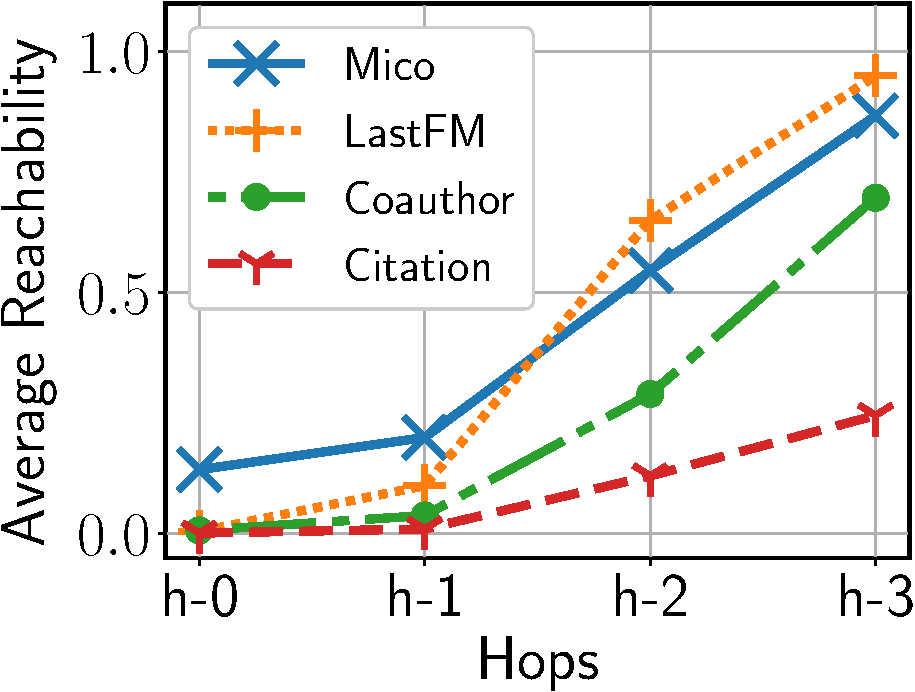
\includegraphics[scale=0.22]{img2/lastfm/lastfm_reachability.pdf}
	\caption{}
	\label{fig:reachability}
	\end{subfigure}%
	\begin{subfigure}[b]{0.21\textwidth}
		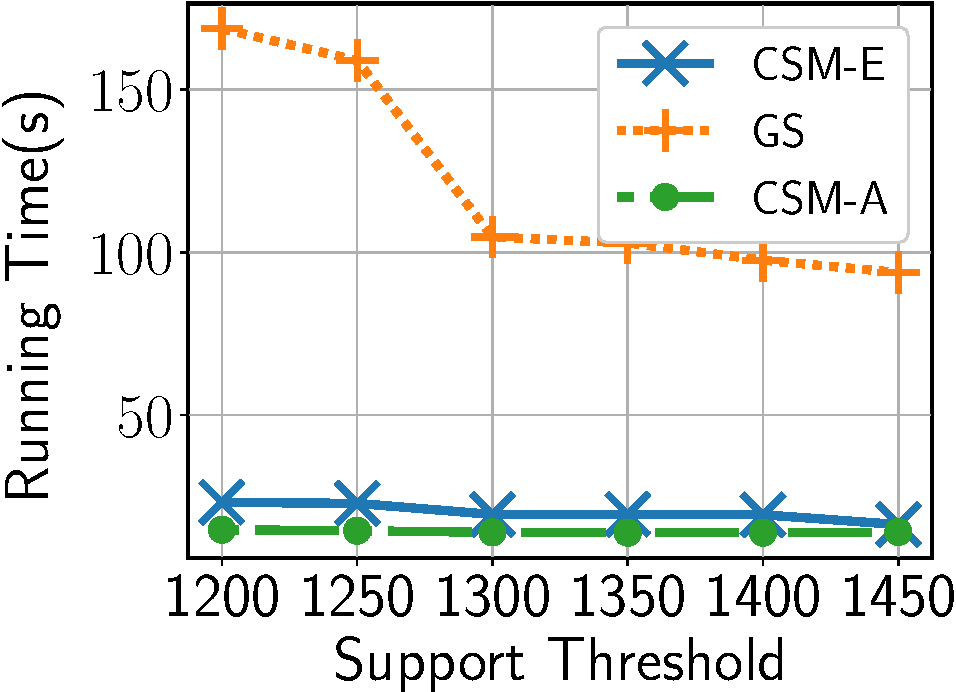
\includegraphics[scale=0.22]{img2/lastfm/lastfm_h1.pdf}
		\caption{{\em LASTFM}}
		\label{fig:lastfm_h1}
	\end{subfigure}%
	\begin{subfigure}[b]{0.21\textwidth}
		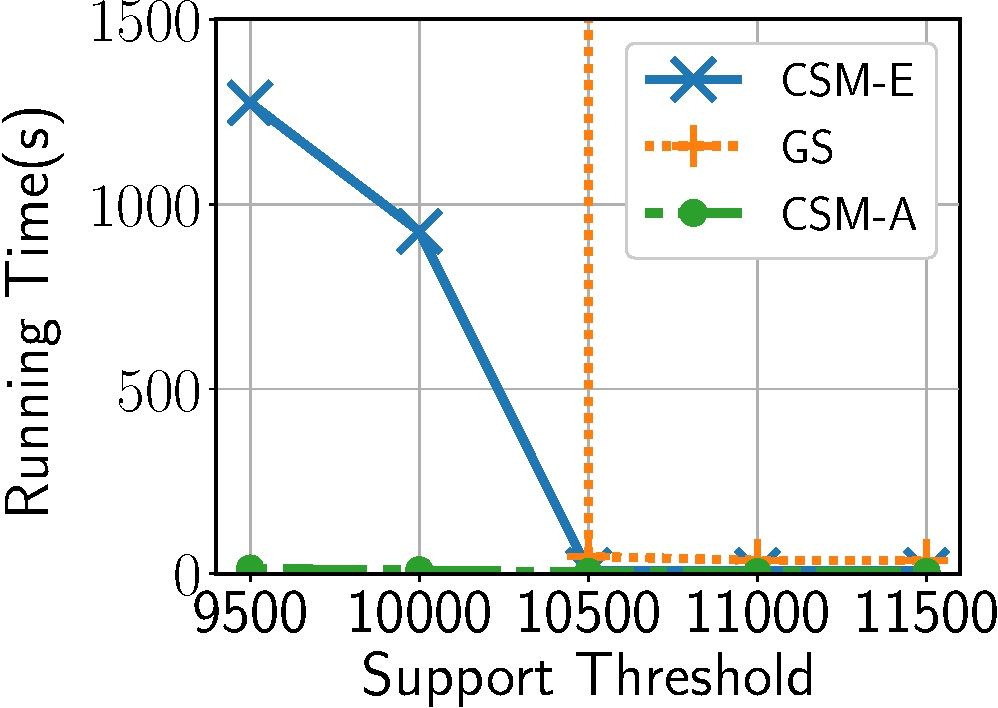
\includegraphics[scale=0.22]{img2/mico/mico_h1.pdf}
		\caption{{\em Mico}}
		\label{fig:mico_h1}
	\end{subfigure}%
	\begin{subfigure}[b]{0.21\textwidth}
		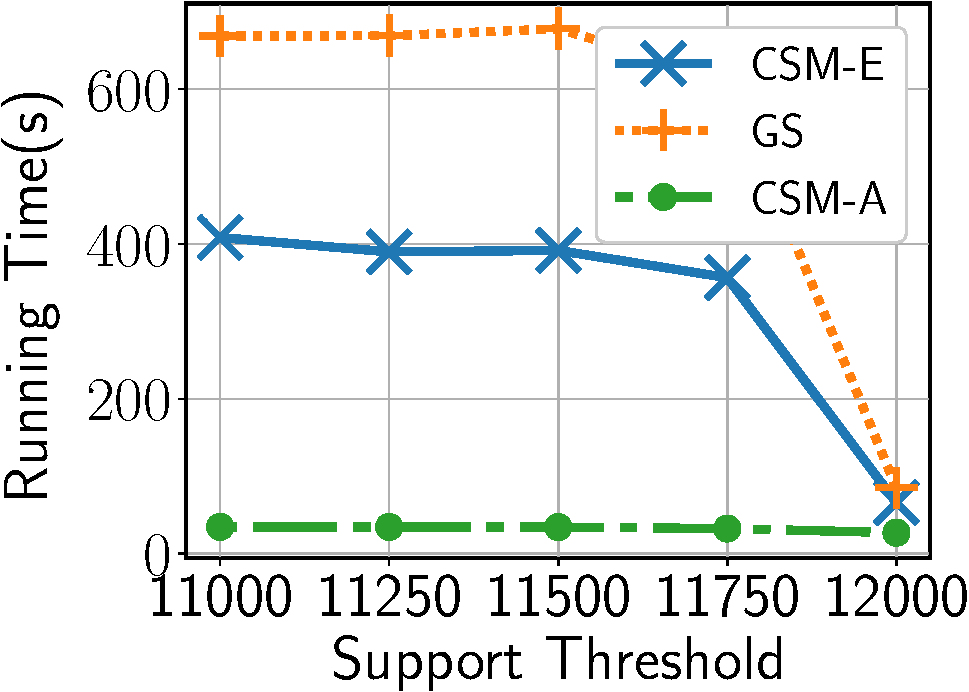
\includegraphics[scale=0.22]{img2/coauthordblp/coauthordblp_h1.pdf}
		\caption{{\em DBLP Coauthor}}
		\label{fig:coauthordblp_h1}
	\end{subfigure}%
	\begin{subfigure}[b]{0.21\textwidth}
		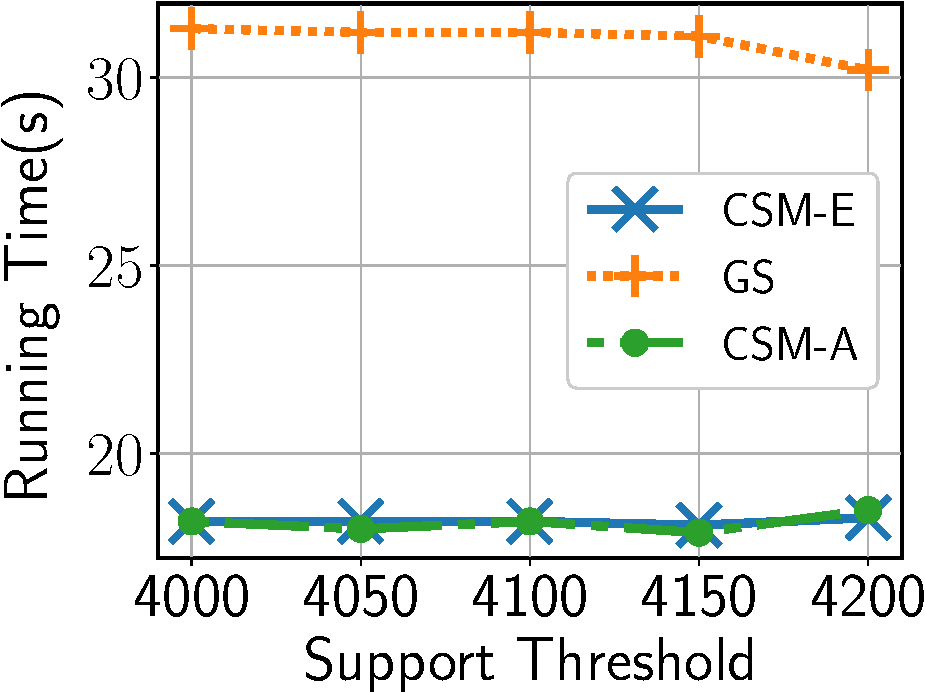
\includegraphics[scale=0.22]{img2/citationdblp/citationdblp_h1.pdf}
		\caption{ {\em DBLP Citation}}
		\label{fig:citationdblp_h1}
	\end{subfigure}%
	\caption{(a) Growth of reachability against $h$. (b-e) Growth of running time against support threshold.}
	\label{fig:baseline_comp}
	\vspace{-1mm}
\end{figure*}
%
\vspace{-0.1in}
\subsubsection{Baselines} We compare {\sf CSM} with two baselines. %The first one is the exact algorithm - \textsc{CSM-Exact} (Section \ref{sec:exact_algo}) . The second one is
%

$\bullet$ \textbf{GraMi+VF3 (GVF3):} This baseline approach has already been discussed in details in \S~\ref{sec:baseline}. %In this approach, we first use \textsc{GraMi}\cite{} to mine frequent subgraphs. Next, we employ the \textsc{VF3}\cite{} to enumerate all instances of the frequent subgraphs and compute the correlation among them to compute the top-$k$ answer set. Both \textsc{GraMi} and \textsc{VF3} are the state-of-the-art algorithms for the specific tasks of mining frequent subgraphs and subgraph enumeration respectively.
%

$\bullet$ \textbf{GrowStore (GS):} \textsc{GrowStore} \cite{KK04} employs the same algorithm as {\sf CSM-E} except one critical difference; instead of using the replica to summarize all instances, we store each of the instances individually. More simply, comparing with \textsc{GrowStore} allows us to precisely quantify the benefit obtained due to using the replica data structure.
%
\vspace{-0.1in}
\subsection{Efficiency}
\label{subsec:efficiency}
%\par \textit{Running Time Comparison.}
We compare the efficiency of {\sf CSM-E} and {\sf CSM-A} against baselines. Since baselines are exorbitantly slow, we %limit ourselves only to the small datasets listed in Table~\ref{tab:datasets}.  for large and dense datasets so we compare the running times of our approximate algorithm with these baselines with
restrict the mining process to only patterns containing at most $5$ nodes. %As the pattern size increases, the cost of enumerating their instances increases exponentially, since it involves performing subgraph isomorphism tests.
%
\begin{table}[b]
	\vspace{-1mm}
		\centering
		\caption{Running Time Efficiency(s)\label{tab:gvf3}}
{\scriptsize
		\begin{tabular} {ccccc}
			\hline
			Datasets  & {\sf CSM-A} & {\sf CSM-E} & \textbf{GVF3}\\			
			\hline
			{\em Chemical}   &   $0.1$    &  $0.1$ & $2.5$\\
			{\em MiCo}   &   $4.5$    &  $8.9$   & $1521$\\
			{\em LastFM}   &   $14$   &  $16.3$ & $346000$\\
			{\em Coauthor(DBLP)}   &   $27.8$    &  $64.3$& $503015$\\
			{\em Citation(DBLP)}   &   $18.2$   &  $18.2$ & $1311474$\\
			{\em Citeseer}   &   $0.1$   &  $0.1$ & $10$\\
			\hline
		\end{tabular}}
	\vspace{-2mm}
\end{table}
\vspace{-0.1in}
\subsubsection{Running time. }
Recall that the running time of {\sf CSM-A} has already been compared with \textbf{GVF3} in the Figure~\ref{fig:motivation}. As visible, {\sf CSM-A} is $5$ orders of magnitude faster than \textbf{GVF3} in the {\em Citation} dataset. The gap in performance is narrower in {\em MiCo} since {\em MiCo} is a much smaller dataset. In Table~\ref{tab:gvf3}, we compare the running times of {\sf CSM-E}, {\sf CSM-A}, and \textbf{GVF3} at the largest possible support threshold such that there is at least one correlated pair. As clearly visible, even when the support thresholds are set at the highest possible values, \textbf{GVF3} is unable to scale in large datasets. For example, {\em in the {\em Citation} dataset, \textbf{GVF3} terminates after $15$ days. In contrast, {\sf CSM-A} and {\sf CSM-E} finish in $18$ seconds. Overall, both the proposed approaches are orders of magnitude faster}.

Next, we compare {\sf CSM-A} and {\sf CSM-E} with \textbf{GS},
to clearly understand the impact of replica. Figures \ref{fig:lastfm_h1}-\ref{fig:citationdblp_h1} present the running times across various datasets. % of the benchmarked algorithms across different datasets against the support threshold. %is varied at $k=20$, $h=1$.
 {\em As expected, {\sf CSM-A} is the fastest algorithm followed by {\sf CSM-E}, and then \textbf{GS}. %Note that we do not show the running time of GraMi-VF3 since it fails to terminate even after $7$ days.
This result shows that replica is effective in reducing the computation cost}. We also observe that {\sf CSM-A} is $10$ times faster than {\sf CSM-E} on average, with the difference being more significant on smaller values of support threshold. This is expected since as the support threshold is lowered, the search space increases exponentially, and the impact of avoiding repetitive computation magnifies.
%
%
%
%
%Several key insights can be derived from Figure \ref{fig:baseline_comp}. %First, as evident from GraMi-VF3, using frequent subgraphs mining to solve the proposed problem is not scalable. Second,
%
\vspace{-0.1in}
\subsubsection{Memory footprint.} Our goal in this experiment is to understand the reduction obtained in memory footprint due to replica. To fully understand the impact of replica, we remove the restriction of mining only patterns of size up to $5$. % Since the baseline algorithms are exorbitantly slow, we %limit ourselves only to the small datasets listed in Table~\ref{tab:datasets}.  for large and dense datasets so we compare the running times of our approximate algorithm with these baselines with restrict the mining process to only patterns containing at most $5$ nodes. %As the pattern size increases, the cost of enumerating their instances increases exponentially, since it involves performing subgraph isomorphism tests.
%Replica provides an efficient mechanism to store all instances of a subgraph pattern in a compact manner. In contrast, \textsc{GrowStore} stores all instances separately. This is a significant bottleneck since, in the worst case, the number of instances of a subgraph could be exponential. %So in a frequent subgraph mining setting, \textsc{GrowStore} does work for small and less dense graphs but as the graph size increases or the graph becomes dense, the number of instances grow exponentially and thus the storage cost becomes too high.
In Figure \ref{fig:citeseer_mem}, we compare the memory footprint of {\sf CSM-A} with \textbf{GS} in {\em Citeseer}. Since {\sf CSM-E} has the same memory requirements as {\sf CSM-A}, we do not show {\sf CSM-E} in Figure \ref{fig:citeseer_mem}.

Without the size restriction of $5$ nodes, \textbf{GS} runs out of memory on large datasets, e.g., in {\em LastFM}, {\em Citation} and {\em Coauthor}, even at high support thresholds. In {\em Citeseer}, which is a small dataset of $4\,500$ edges, \textbf{GS} consumes more than $10GB$ of main memory at support threshold of $175$; and at the lowest support threshold of $150$, it exceeds $256GB$. {\em In contrast, the memory footprint of {\sf CSM-A} is $100$ times lower on average}. The memory consumption grows with reduction in support thresholds since more subgraphs become frequent. Overall, the stark difference in memory consumption between {\sf CSM-A} and \textbf{GS} highlights the benefit of replica on memory footprint.% In the plot of LastFM, we have just one point %
\vspace{-0.1in}
\subsection{Approximation Quality}
\label{sec:quality}
We evaluate the approximation quality of {\sf CSM-A} by comparing it with the top-$k$ answer set of {\sf CSM-E} (ground-truth). The accuracy of {\sf CSM-A} is quantified with three metrics: %Jaccard coeeficient\cite{}, and measure the accuracy ofWe show the quality of our approximation algorithm by comparing the results of top k of our approximate algorithm with the exact version, both run with a size bound of maximum 5 sized patterns. We take the output of the complete version as the ground truth for all the experiments. The following 3 experiments are done to show quality of our approximate version:
% \newline

$\bullet$ \textbf{Jaccard Coefficient} \cite{jaccard}: Jaccard coefficient measures the similarity of the approximate answers with the ground truth. %Jaccard coefficient ranges from $0$ to $1$, with $1$ indicating exact match.%ion of pairs that we have in the approximate output which are there in the ground truth as well. The fraction comes out to be $1$ for all the datasets which means we get the exact same results as the exact version.

$\bullet$ \textbf{Kendall's Tau} \cite{kendall}: Kendall's Tau measures how accurately the ranking of the patterns in the ground truth is preserved in the top-$k$ answer set of {\sf CSM-A}. %This is a measure of relationships between ranked data and focusses on the ordering of the results.
It ranges from $0$ to $1$, with $1$ indicating perfect preservation of the ranking order. %It is calculated as \[KT = \dfrac{C-D}{C+D}, C = |concordant\ pairs|, D = |disconcordant\ pairs|\] Concordant pairs are how many larger ranks are below a certain rank and disconcordant pairs are how many smaller ranks are below a certain rank. We keep $K-20$ and show results of varied $hops$ at different supports for $LastFM$ in Figure \ref{fig:lastfm_kt}.\\

$\bullet$ \textbf{Percentage error in correlation count.} This metric measures the error in correlation count introduced by the approximate version. The percentage error for a given pattern $p$ is $\frac{\kappa^*_p-\kappa_p}{\kappa^*_p}\times 100$, where $\kappa_p$ is the correlation count for the pair of subgraphs $p$ in {\sf CSM-A} and $\kappa^*_p$ is the exact value in CSM-E for this same pair. From Lemma~\ref{lem:lowerbound}, we are guaranteed that $\kappa^*_p\geq\kappa_p$ for any pattern $p$. We compute the  percentage error across all common top-$k$ patterns in the approximate and the exact set and report the mean error (in percentage).

 We report the accuracies across all datasets in Table \ref{tab:quality}. %The support threshold for every dataset is taken as the minimum support for the support ranges chosen in Fig.~\ref{fig:support}.
{\em As can be seen, {\sf CSM-A} produces near-optimal results}. %This is expected since as established in Theorem~\ref{thm:homomorphism}, inaccuracy creeps in only in some special cases of homomorphism. Such cases are rare in real graphs, and consequently, we observe excellent performance.
To further analyze how the quality changes with support threshold, in Figures~\ref{fig:lastfm_error} and \ref{fig:lastfm_kt}, we plot the percentage error and Kendall's Tau against support for various values of $h$. {\em Consistent with previous observations, the results remain near-optimal throughout}. %in  shows this error at $K-20$ and varied $hops$ at different supports for LastFM.
We do not include Jaccard Coefficient in this experiment since it is always $1$. Due to space limitations, we show the result only in {\em LastFM}. Similar trends are observed across all datasets. %These results show that the accuracy is robust to parameter variation.
%
\begin{table}[tb!]
	\begin{center}
		\centering
		\caption{Quality evaluation of CSM-A\label{tab:quality}}
{\scriptsize
		\begin{tabular} {ccccc}
			\hline
			Datasets  & Jaccard Coeff & Kendall's Tau  & Percentage Error & Support\\			
			\hline
			{\em Chemical}   &   $1.0$   &  $1.0$   & $0$ & $10$\\
			{\em Yeast}   &   $1.0$    &  $1.0$  & $0$ & $300$\\
			{\em MiCo}   &   $1.0$    &  $1.0$   & $0$ & $9500$\\
			{\em LastFM}   &  $1.0$   &  $1.0$ & $0$ & $1200$\\
			{\em Coauthor(DBLP)}   &   $1.0$  &  $0.98$  & $2.26$ & $11000$\\
			{\em Citation(DBLP)}   &   $1.0$   &  $1.0$   & $0$ & $4000$\\
			{\em Citeseer}   &   $1.0$   &  $1.0$ & $0$ & $150$\\
			
			\hline
		\end{tabular}}
	\end{center}
	\vspace{-1mm}
\end{table}
%
\begin{figure*}
	\vspace{4mm}
	\centering
	\begin{subfigure}[b]{0.25\textwidth}
		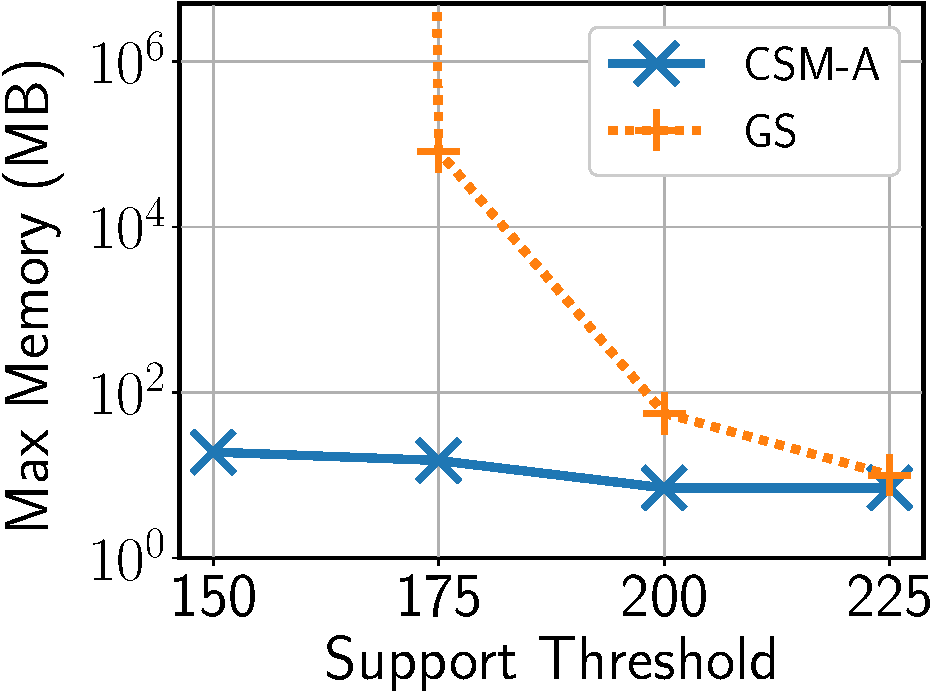
\includegraphics[keepaspectratio,scale=0.24]{img2/citeseer/citeseer_mem.pdf}
		\caption{{\em Citeseer}}
		\label{fig:citeseer_mem}
	\end{subfigure}%
	\begin{subfigure}[b]{0.25\textwidth}
		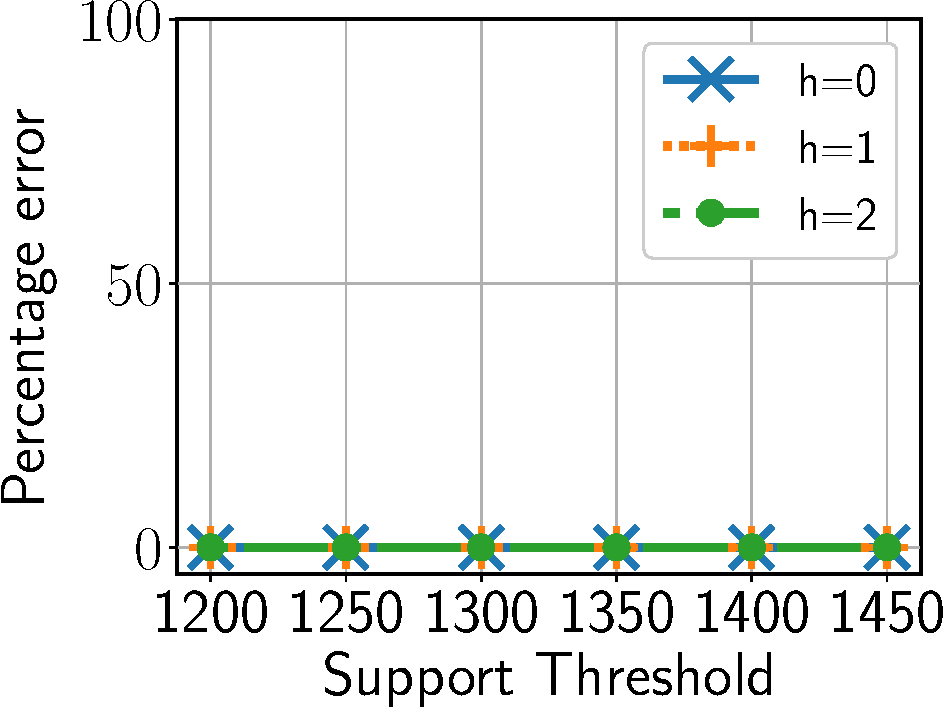
\includegraphics[keepaspectratio,scale=0.24, angle=0]{img2/lastfm/lastfm_spread.pdf}
		\caption{{\em LastFM}}
		\label{fig:lastfm_error}
	\end{subfigure}%
	\begin{subfigure}[b]{0.25\textwidth}
		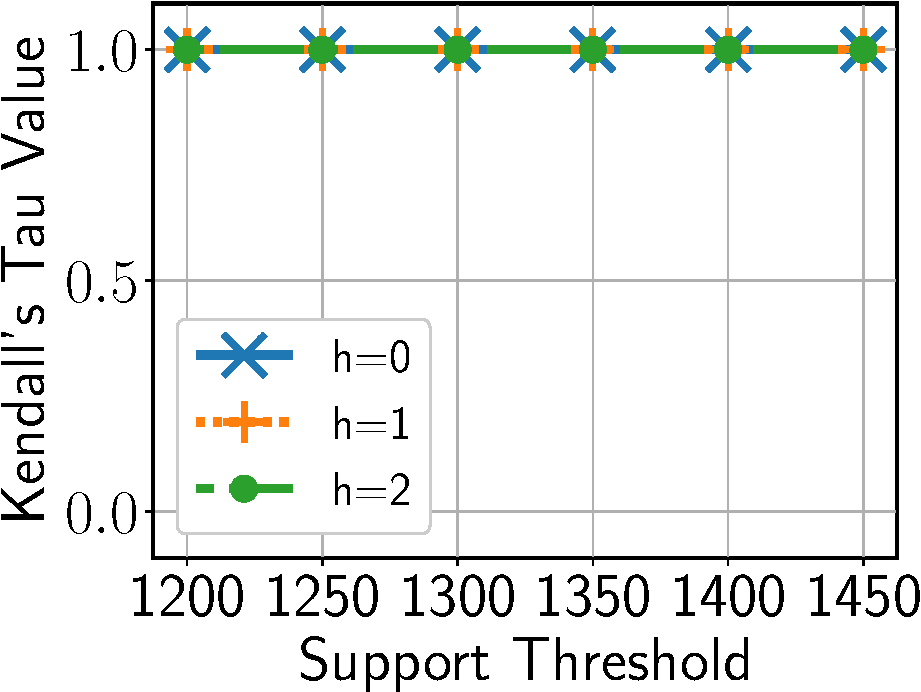
\includegraphics[keepaspectratio,scale=0.24, angle=0]{img2/lastfm/lastfm_kt.pdf}
		\caption{{\em LastFM}}
		\label{fig:lastfm_kt}
	\end{subfigure}%
\begin{comment}
	\begin{subfigure}[b]{0.25\textwidth}
		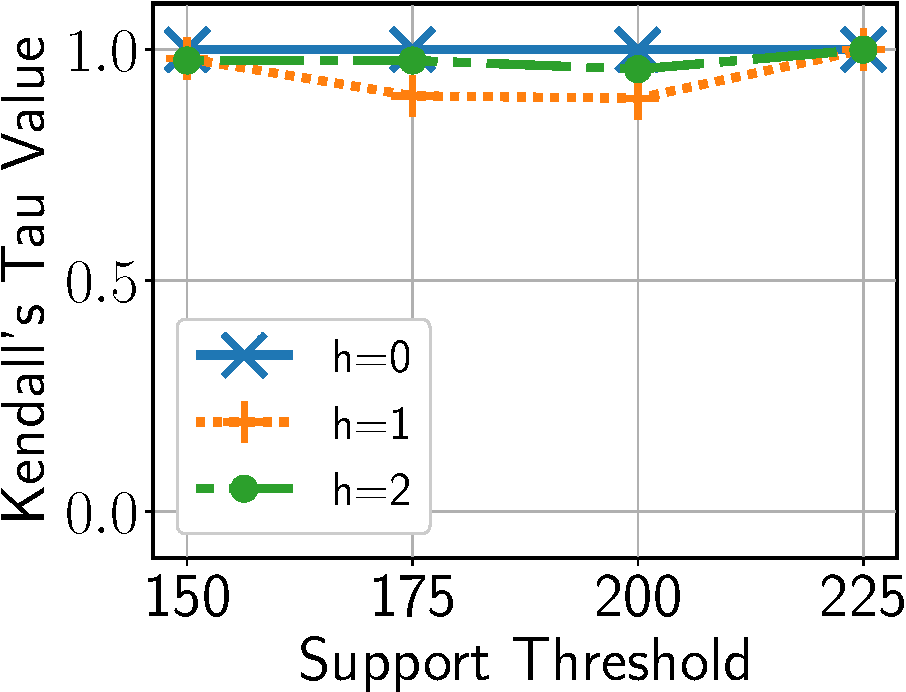
\includegraphics[keepaspectratio,scale=0.21, angle=0]{img2/citeseer/citeseer_kt.pdf}
		\caption{{\em Citeseer}}
	\end{subfigure}%
	\begin{subfigure}[b]{0.22\textwidth}
		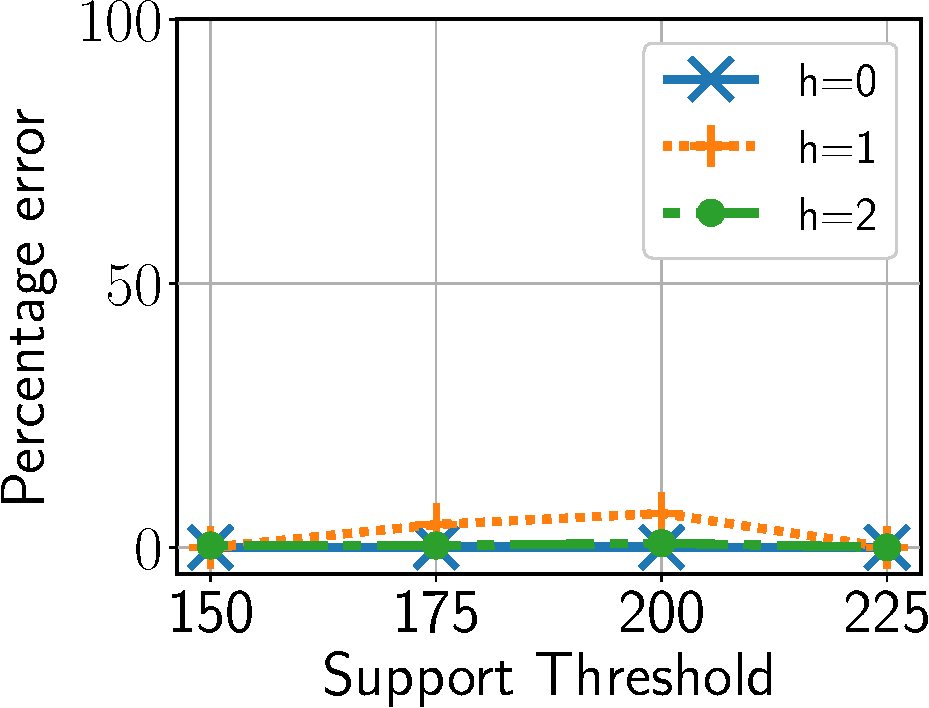
\includegraphics[keepaspectratio,scale=0.21, angle=0]{img2/citeseer/citeseer_spread.pdf}
		\caption{{\em Citeseer}}
		\label{fig:citeseer_error}
	\end{subfigure}
\end{comment}
	\begin{subfigure}[b]{0.25\textwidth}
		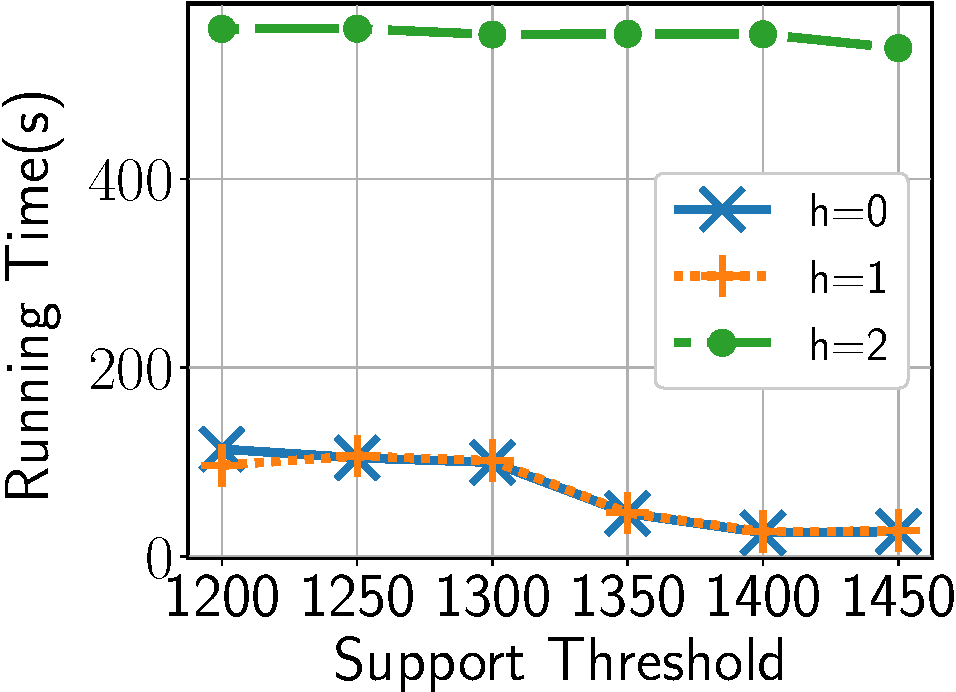
\includegraphics[keepaspectratio, scale=0.24, angle=0]{img2/lastfm/lastfm_running_time_nobound.pdf}
		\caption{{\em LastFM}}
		\label{fig:lastfm_nosb}
	\end{subfigure}\\
	\begin{subfigure}[b]{0.25\textwidth}
		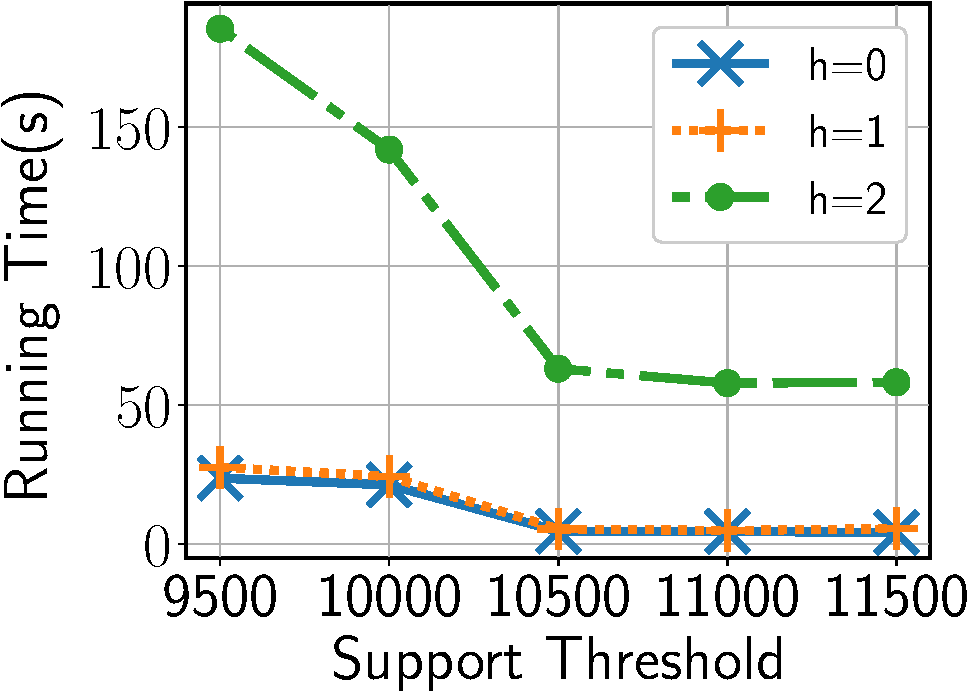
\includegraphics[keepaspectratio, scale=0.24, angle=0]{img2/mico/mico_running_time_nobound.pdf}
		\caption{{\em Mico}}
		\label{fig:mico_nosb}
	\end{subfigure}%
	\begin{subfigure}[b]{0.25\textwidth}
		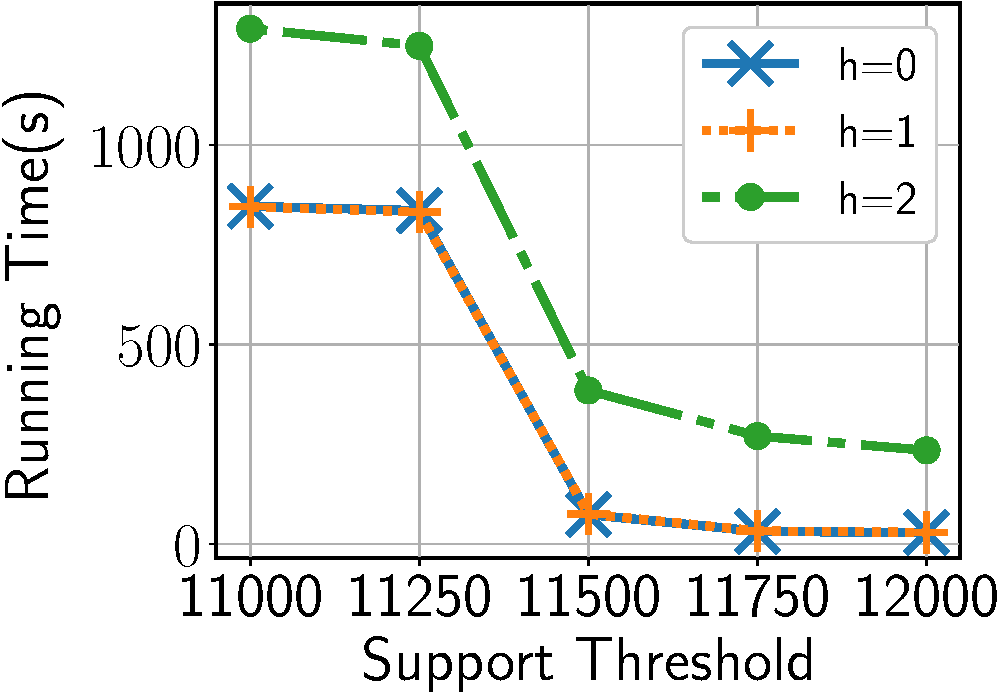
\includegraphics[keepaspectratio, scale=0.24, angle=0]{img2/coauthordblp/coauthordblp_running_time_nobound.pdf}
		\caption{{\em DBLP Coauthor}}
		\label{fig:coauthordblp_nosb}
	\end{subfigure}%
	\begin{subfigure}[b]{0.25\textwidth}
		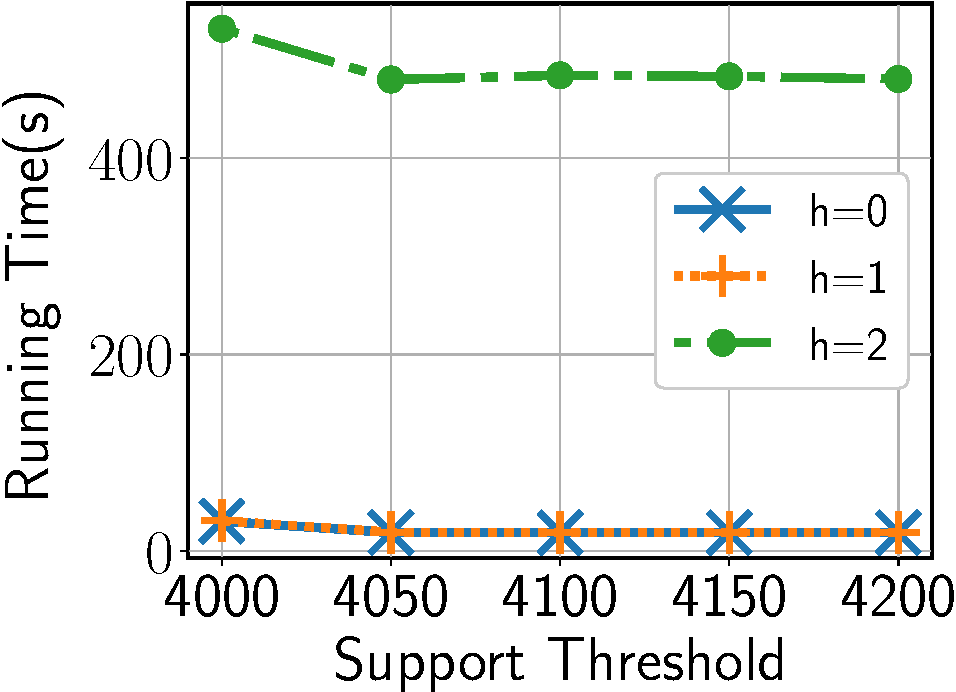
\includegraphics[scale=0.24, angle=0]{img2/citationdblp/citationdblp_running_time_nobound.pdf}
		\caption{{\em DBLP Citation}}
		\label{fig:citation_nosb}
	\end{subfigure}%
	\begin{subfigure}[b]{0.25\textwidth}
		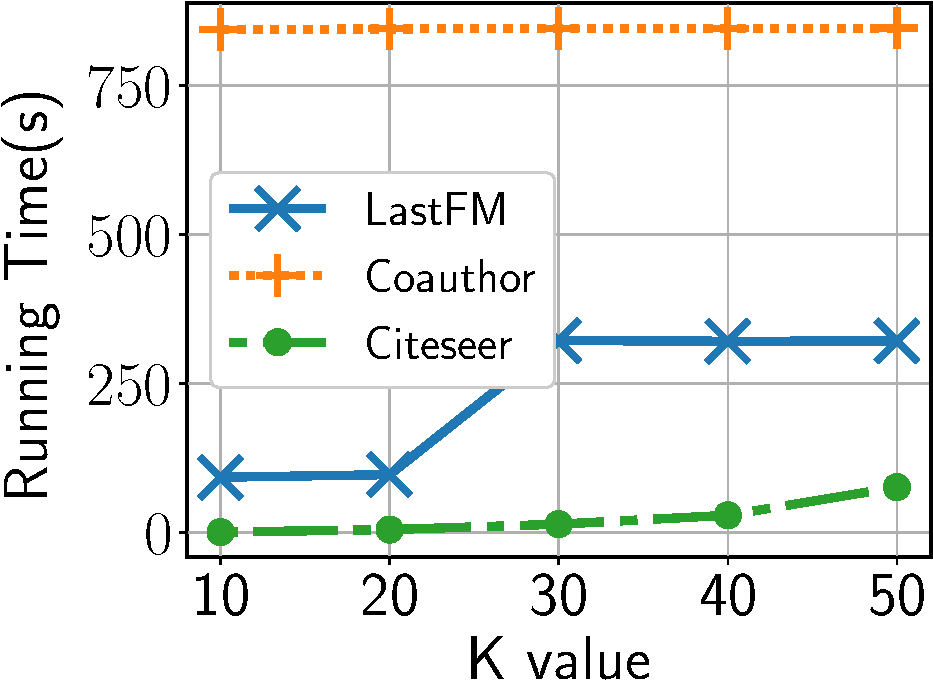
\includegraphics[keepaspectratio,scale=0.25]{img2/lastfm/lastfm_K_var_fnl.pdf}
		\caption{}
		\label{fig:lastfm_k}
	\end{subfigure}%
	\caption{(a) Growth of memory consumption against support threshold. (b-c) Approximation quality of {\sf CSM-A} against support threshold. (d-e) Growth rate of {\sf CSM-A}'s running time against: (d-g) support threshold and (h) $k$. For (h) the support thresholds are as follows: {\em LastFM}: $1200$, {\em DBLP Coauthor}:$11000$, {\em Citeseer}: $150$. }
	\label{fig:quality}
	\vspace{-1mm}
\end{figure*}
%
\vspace{-0.1in}
\subsection{Impact of Parameters}
After establishing that {\sf CSM-A} is accurate and fast, we measure its scalability on large graphs against various parameters.

\vspace{-0.1in}
\subsubsection{Running Time.} In \S~\ref{subsec:efficiency}, we had to limit the mining process only to patterns of size up to $5$ due to the non-scalability of the baseline algorithms. In the next set of experiments, we remove this constraint and measure the growth rate of running time against the support threshold. In addition, we also plot the running times across all values in the range $h\in [0,2]$. Figures~\ref{fig:lastfm_nosb}-\ref{fig:citation_nosb} present the results in the four largest datasets listed in Table~\ref{tab:datasets}. As expected, the running time decreases with increasing support. {\em What is more noteworthy is that even at $h=2$, {\sf CSM-A} terminates within $20$ minutes on million-scale datasets}. As we increase $h$, time and space required to compute proximate nodes' index ($CorV$) increases and as a result, the time taken for correlation computation also increases due to more correlations obtained. %However, this can sometimes lead to early termination as the top-$k$ set gets filled early. If the decrease in time due to this dominates the increase in time which is there, time may also decrease with increasing hops.
% From our empirical result, if there are enough $k$ correlations eligible, the time cost of all the datasets setting $h=0$ and $h=1$ could have no difference larger than $1$ sec. This is because through $h=1$ has a time increase from $h=0$, the total time cost at correlation calculation still does not dominate the total time cost. However, setting $h=2$ would receive a much higher time cost because the time cost of correlation calculation begins to dominate the total cost. However, when $h=3$, the time cost becomes extremely expensive and also has the memory cost over $256$GB. As a result, an approximation mining approach need to be proposed.
%
%CSM-A peak memory usage results w/ varying hops:


Figure \ref{fig:lastfm_k} analyzes the growth rate of running time against $k$. As $k$ increases, it is expected that more patterns will be processed and hence the running time should increase. The increase, however, is minimal since in proportion to the number of subgraphs in the search space, $k$ is very small. %However, it might happen that for a chosen support, the program is terminated after all the patterns are processed and there is no pattern remaining in the {\sf Search\ Queue} which means we cannot get more correlated patterns if we increase k. The time in such cases would stay the same after a certain K as can be seen in the case of $DBLP Coauthor$.

% \par Also, we provide the {\sf Top-$3$} correlations of datasets {\em (1)(2)(3)(4)} in Figure \ref{fig:tp} and give an example for the analysis of some results. As in Figure \ref{fig:tp_lastfm}, the result shows that {\em Coldplay} is a popular band and people who like {\em Coldplay} are very likely to have some friends who like {\em Coldplay} as well. Besides, people who like {\em Radiohead} are very likely to be in the social group where many people like {\em Coldplay}.


\vspace{-0.1in}
\subsubsection{Memory footprint.} Figure \ref{fig:mem_hops} analyzes the memory footprint against support threshold for various values of $h$. Two key trends emerge. First, {\em as support decreases, the increase in memory consumption of CSM-A is minimal. This follows from the property that CSM-A maintains only replicas at any point of time}. The small increase in memory results from storing more subgraph patterns (but not their instances). As $h$ increases, the memory required to store the proximate nodes index, which stores all frequent nodes within $h$ hops from each frequent node, goes up.

\vspace{-0.1in}
\subsubsection{Search Strategy.} We adopt  $Best$-$First$ $Search (BEST)$ strategy to explore the search space. How would the performance be if we adopt $Breadth$-$First$ $Search (BFS)$ or $Depth$-$First$ $Search (DFS)$? Our next experiment answers this question. More specifically, we explore the search space using each of these strategies and track their pruning power by counting the number of patterns popped from the {\sf Search\ Queue}. We use this methodology instead of comparing the running time since this is more precise and hardware-independent.

Figure \ref{fig:dbfs} presents the results against $k$. {\em BEST is built on the observation that subgraphs with higher frequency tend to have a higher correlation with other frequent subgraphs. This prioritization scheme yields better results across most datasets}. Specifically, the results obtained in {\em LastFM}  and {\em Chemical} reflect the trends in other datasets as well; we omit them due to space limitations.
%\textcolor{blue}{However, we see that all three strategies produce similar running times in $LastFM$ for higher supports. On analyzing this phenomenon further, we discover that in $LastFM$, at higher supports, the algorithm terminates when the search queue gets empty, which means all three strategies explore all possible patterns. In the other datasets, the algorithm terminates due to hitting the Ceasing condition (Sec.~\ref{subsubsec:exact_algo_ceasing}), which guarantees that all unexplored patterns in the queue are guaranteed to not be in the top-$k$ answer set. Overall, we observe that BEST is generally faster and never worse than BFS or DFS.}

%\par In $DFS$, if we go to a branch where all patterns are frequent till a greater depth, it will lead to a lot of patterns being processed. $BFS$ processes all the patterns at a level as we can only stop processing patterns when all the patterns at a given depth have support less than the least correlation value in top k. However in best first search, there is no such restriction and we can stop as soon as we find a pattern with support less than the least correlation value in top k as all the other patterns will have a support less than or equal to the current pattern. In addition, the problem setting is such that patterns with higher frequency tend to have a higher correlation with other patterns and the best first strategy takes full advantage of this. However, if program gets terminated after all the patterns are processed and there are no patterns remaining in the {\sf Search\ Queue}, best first will have exactly same number of patterns explored as $BFS$ and $DFS$.

\eat{
\begin{figure}[t!]
\vspace{4mm}
\centering
\subfigure[{\scriptsize {\sf K}=$20$, $Hop=1$ in {\em LastFM}}] {
\includegraphics[keepaspectratio,scale=0.24, angle=0]{img2/lastfm/lastfm_bfsdfs_pop.pdf}
\label{fig:lastfm_bfsdfs_pop}
}
\subfigure[{\scriptsize {\sf Sup}=$1200$, $Hop=1$ in {\em LastFM}}] {
\includegraphics[keepaspectratio,scale=0.24, angle=0]{img2/lastfm/lastfm_bfsdfs_pop_k.pdf}
\label{fig:lastfm_bfsdfs_pop_k}
}
\subfigure[{\scriptsize {\sf K}=$20$, $Hop=1$ in {\em Chemical}}]  {
\includegraphics[keepaspectratio,scale=0.24, angle=0]{img2/chemical/chemical_bfsdfs_pop.pdf}
\label{fig:chemical_bfsdfs_pop}
}
\subfigure[{\scriptsize{\sf Sup}=$10$, $Hop=1$ in {\em Chemical}}]  {
\includegraphics[keepaspectratio,scale=0.24, angle=0]{img2/chemical/chemical_bfsdfs_pop_k.pdf}
\label{fig:chemical_bfsdfs_pop_k}
}

\subfigure[{\scriptsize {\sf K}=$20$, $Hop=1$ in {\em DBLP Citation}}]  {
\includegraphics[keepaspectratio,scale=0.24, angle=0]{img2/citationdblp/citationdblp_bfsdfs_pop.pdf}
\label{fig:chemical_bfsdfs_pop}
}
\subfigure[{\scriptsize{\sf Sup}=$10$, $Hop=1$ in {\em DBLP Citation}}]  {
\includegraphics[keepaspectratio,scale=0.24, angle=0]{img2/citationdblp/citationdblp_bfsdfs_pop_k.pdf}}
\label{fig:chemical_bfsdfs_pop_k}
\vspace{-2mm}
\caption{Performance of different search strategies.}
\label{fig:dbfs}
\vspace{-2mm}
\end{figure}
}


% \spara{$\bullet$ Index Analysis} We provide the result of efficiency increase of our global index. The index strategy is more powerful if there are fewer distinct edge labels or the data graph is more dense, like {\em Yeast} and {\em DBLP}.


% \begin{figure}[t!]
% \vspace{4mm}
% \centering
% \subfigure[{\scriptsize {\em Chemical} with {\sf Min-sup} = $10$, $k=50$}] {
% \includegraphics[scale=0.17, angle=270]{img2/ni_chemical}
% \label{fig:ni1}
% }
% \subfigure[{\scriptsize {\em Yeast} with {\sf Min-sup} = $200$, $k=50$}]  {
% \includegraphics[scale=0.17, angle=270]{img2/ni_yeast}
% \label{fig:ni2}
% }
% \subfigure[{\scriptsize {\em DBLP} with {\sf Min-sup} = $5000$, $k=50$}] {
% \includegraphics[scale=0.17, angle=270]{img2/ni_dblp}
% \label{fig:ni3}
% }
% \subfigure[{\scriptsize {\em LastFM} with {\sf Min-sup} = $200$, $k=50$}]  {
% \includegraphics[scale=0.17, angle=270]{img2/ni_lastfm}
% \label{fig:ni4}
% }
% \vspace{-2mm}
% \caption{\scriptsize Figure for index analysis.}
% \label{fig:ni}
% \vspace{-2mm}
% \end{figure}
%
\vspace{-0.1in}
\subsection{Application}
\label{sec:application}

% \textit{Yeast}\cite{yeast_source}
%An application of the \textsc{CSM} model on biological networks reveals
%interesting structural correlations among biological substructures that mirror
%the correlation observed in their biological functioning.
%  and provides insights
% into structures of correlated patterns that
% probably give rise to such correlative functioning.
To demonstrate the utility of mining correlated subgraph pairs, we present insights derived from mining correlated pairs on the \emph{Yeast} \cite{yeast_source} dataset.
%, a Protein-Protein Interaction (PPI) network(\S~\ref{ref:datasets}): \textbf{(1)} \emph{Function},
%and \textbf{(2)} \emph{Process} graph. \emph{Yeast Function}
The node labels (Gene Ontology tags) in this Protein-Protein Interaction (PPI) network (\S~\ref{ref:datasets}) indicate their  biological activity. % of the %nodes based
%on elemental activities performed by the node at a molecular level while
%\emph{Yeast Process} tags nodes with the associated biological process (i.e.
%sets of molecular events). We execute \textsc{CSM-A} on both graphs with $h=1$
 In Figure~\ref{fig:yeast} we present two of the top-$20$ correlated pairs mined at $\Sigma=300$. Figures \ref{fig:f1} ($Q_1$) and~\ref{fig:f2} ($Q_2$) present the first pair. %, an interesting pair mined in \emph{Yeast Function}.
%With $\kappa(Q_1, Q_2,h=1)=383$, the pair is ranked second among the top-$20$ pairs.
$Q_1$ is constituted entirely of units specialising in \emph{ion
binding}, while $Q_2$ is composed of those specialising in \emph{transferase
activity}. Keike et al.\cite{pattern1,pattern2} show that transferases gain
enzymatic activity following the binding of ionic ligands, undergoing
conformational changes to insulate the ligands from surrounding water molecules.
The frequent co-occurrence of these subgraph patterns specializing in two complementary biological
functions shows that the proposed model is effective in discovering semantically meaningful associations. Furthermore, this is a pattern that frequent subgraphs mining techniques would not identify.%supports the above observations that the functions are complementary.
%Moreover, it goes a step further in suggesting the structural configuration of
%both protein structures - the interaction among which enables the activation of
%such an enzymatic activity.

%Similarly, in \emph{Process} PPI network,
We highlight another pair $(Q_3,Q_4)$ in Figures~\ref{fig:p1} and \ref{fig:p2}.
%$\kappa(Q_3,Q_4,h=1)=311$ and rank $3$.
$Q_3$ is  made up of genes that handle responses to {\em chemicals}, while $Q_4$ is
associated with {\em transcription}. This co-occurrence is not a coincidence. Specifically, the Gene Ontology\cite{pattern3} database
 describes in detail the involvement of positive transcription
regulation in cellular response to chemical stimulus. %Perhaps the
%structual configuration of the proteins associated with these biological
%processes in which they frequently co-occur are correlated to the biological
%function performed in conjunction.
%
\begin{figure}[b]
	% \vspace{-2mm}
	\centering
	\begin{subfigure}[b]{0.25\textwidth}
		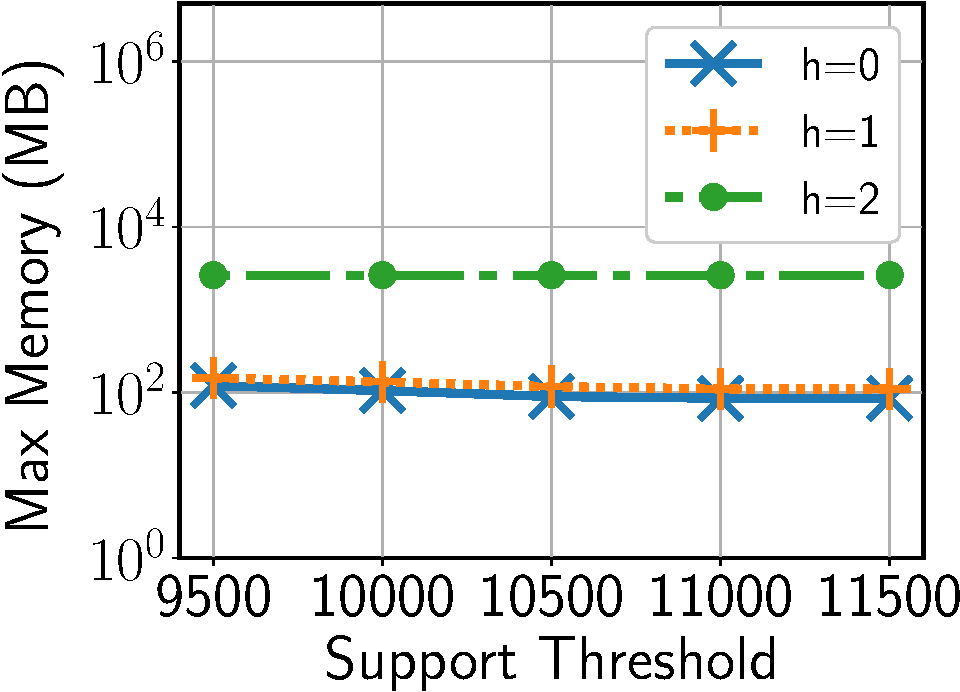
\includegraphics[scale=0.24]{img2/mico/mico_mem_hops.pdf}
		\caption{\scriptsize $Mico$}
		\label{fig:mico_mem_hops}
	\end{subfigure}%
	\hspace*{\fill}
	\begin{subfigure}[b]{0.25\textwidth}
		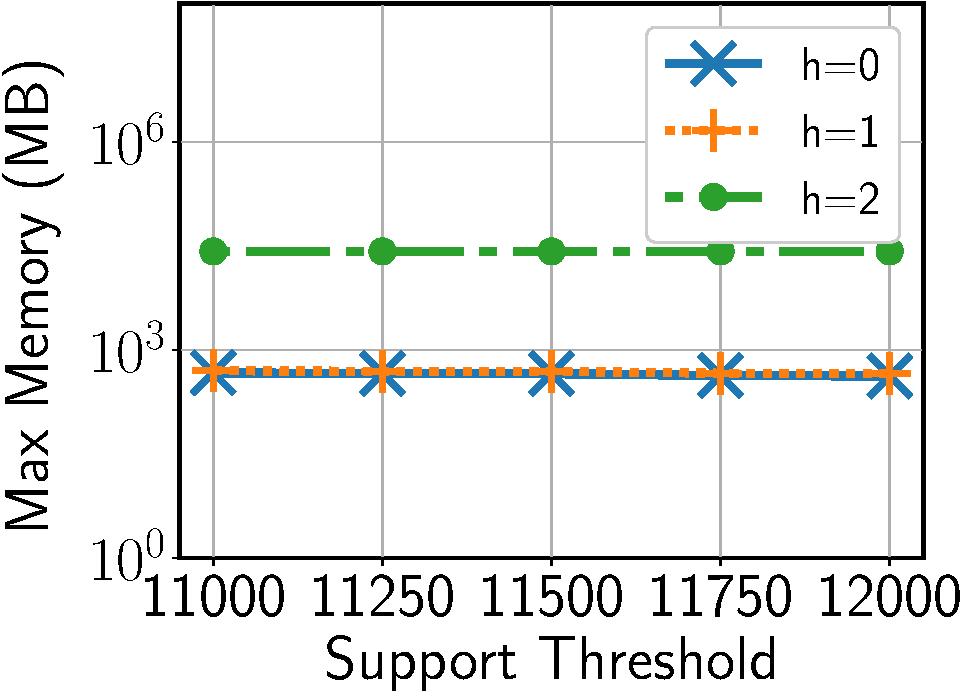
\includegraphics[scale=0.24]{img2/coauthordblp/coauthordblp_mem_hops.pdf}
		\caption{\scriptsize $Coauthor(DBLP)$}
		\label{fig:coauthor_mem_hops}
	\end{subfigure}%
	% \begin{subfigure}[b]{0.25\textwidth}
	% 	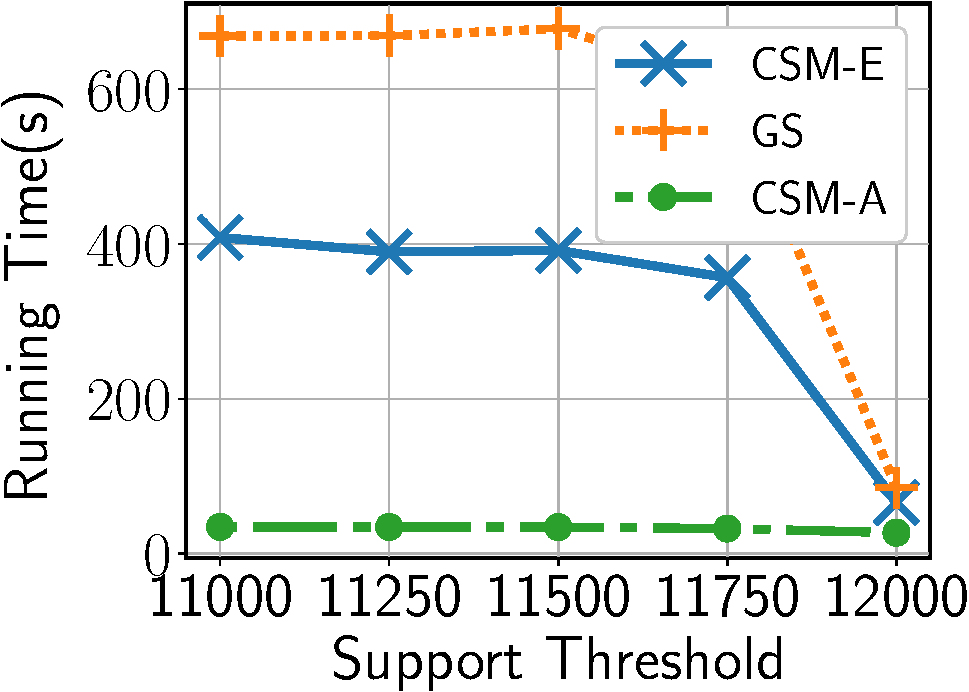
\includegraphics[scale=0.24]{img2/coauthordblp/coauthordblp_h1.pdf}
	% 	\caption{\scriptsize {\sf Hop-$1$, K-$20$} in {\em DBLP Coauthor}}
	% 	\label{fig:coauthordblp_h1}
	% \end{subfigure}%
	% \begin{subfigure}[b]{0.25\textwidth}
	% 	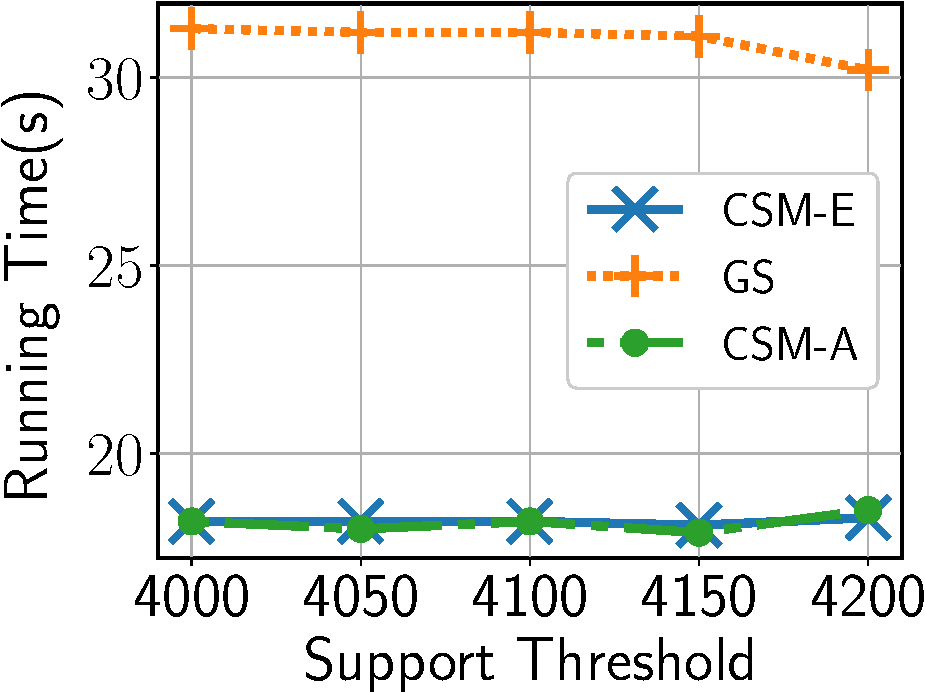
\includegraphics[scale=0.24]{img2/citationdblp/citationdblp_h1.pdf}
	% 	\caption{\scriptsize {\sf Hop-$1$, K-$20$} in {\em DBLP Citation}}
	% 	\label{fig:citationdblp_h1}
	% \end{subfigure}%
	\caption{Memory usage of {\sf CSM-A} against support threshold at different values of $h$.}
	\label{fig:mem_hops}
	\vspace{-3mm}
\end{figure}
\begin{figure}[b]
	\centering
\begin{comment}
	\begin{subfigure}[b]{0.25\textwidth}
		\includegraphics[keepaspectratio,scale=0.24, angle=0]{img2/lastfm/lastfm_bfsdfs_pop.pdf}
		\caption{\scriptsize {\sf K}=$20$, $Hop=1$ in {\em LastFM}}
		\label{fig:lastfm_bfsdfs_pop}
	\end{subfigure}%
\end{comment}
	\begin{subfigure}[b]{0.25\textwidth}
		\includegraphics[keepaspectratio,scale=0.24, angle=0]{img2/lastfm/lastfm_bfsdfs_pop_k.pdf}
		\caption{\scriptsize {\sf Sup}=$1200$, $h=1$ in {\em LastFM}}
		\label{fig:lastfm_bfsdfs_pop_k}
	\end{subfigure}%
\begin{comment}
	\begin{subfigure}[b]{0.25\textwidth}
		\includegraphics[keepaspectratio,scale=0.24, angle=0]{img2/chemical/chemical_bfsdfs_pop.pdf}
		\caption{\scriptsize {\sf K}=$20$, $Hop=1$ in {\em Chemical}}
		\label{fig:chemical_bfsdfs_pop}
	\end{subfigure}%
\end{comment}
	\begin{subfigure}[b]{0.25\textwidth}
		\includegraphics[keepaspectratio,scale=0.24, angle=0]{img2/chemical/chemical_bfsdfs_pop_k.pdf}
		\caption{\scriptsize{\sf Sup}=$10$, $h=1$ in {\em Chemical}}
		\label{fig:chemical_bfsdfs_pop_k}
	\end{subfigure}
% 	\begin{subfigure}[b]{0.25\textwidth}
% 		\includegraphics[keepaspectratio,scale=0.24, angle=0]{img2/citationdblp/citationdblp_bfsdfs_pop.pdf}
% 		\caption{\scriptsize {\sf K}=$20$, $Hop=1$ in {\em DBLP Citation}}
% 		\label{fig:citation_bfsdfs_pop}
% 	\end{subfigure}%
% 	\begin{subfigure}[b]{0.25\textwidth}
% 		\includegraphics[keepaspectratio,scale=0.24, angle=0]{img2/citationdblp/citationdblp_bfsdfs_pop_k.pdf}
% 		\caption{\scriptsize{\sf Sup}=$10$, $Hop=1$ in {\em DBLP Citation}}
% 		\label{fig:citation_bfsdfs_pop_k}
% 	\end{subfigure}%	
	\vspace{-2mm}
	\caption{Performance of different search strategies.}
	\label{fig:dbfs}
	\vspace{-2mm}
\end{figure}

% \begin{figure}
% 	\centering
% 	\subcaptionbox{%
% 		A a $20\times 20$ image in original size.
% 	  }[0.45\linewidth]
% 	  {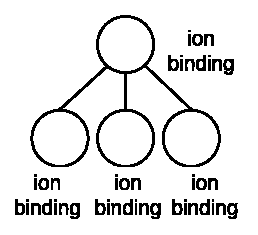
\includegraphics[scale=0.6]{img_ex/func_1.pdf}}
% 	\hfill
% 	\subcaptionbox{%
% 		The same images with increased resolution, for illustrative purposes.
% 	  }[0.54 \linewidth]
% 	  {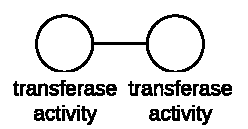
\includegraphics[scale=0.6]{img_ex/func_2.pdf}}
% 	\end{figure}
%
\begin{figure}[tb!]
	\vspace{-0.20in}
	\centering
	\begin{subfigure}[b]{0.12\textwidth}
		% \centering
	% \hspace*{0.9mm}
	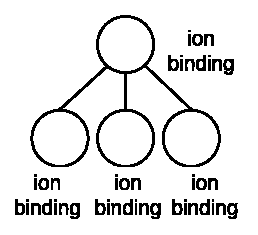
\includegraphics[scale=0.5]{img_ex/func_1.pdf}
	\caption{Pattern $Q_1$}
		\label{fig:f1}
	\end{subfigure}%
% \captionsetup[subfigure]{labelfont=bf,textfont=normalfont,singlelinecheck=on,justification=raggedright, skip=-5pt}
	\begin{subfigure}[b]{0.30\textwidth}
		% \centering
		\hspace*{15mm}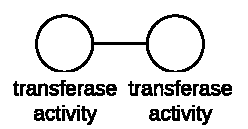
\includegraphics[scale=0.6]{img_ex/func_2.pdf}
		% \vspace{-4.5mm}
		\caption{Pattern $Q_2$}
		\label{fig:f2}
	\end{subfigure}

	% \hspace*{0.25cm}
	\begin{subfigure}[b]{0.12\textwidth}
		% \centering
	\hspace*{-5.9mm}
	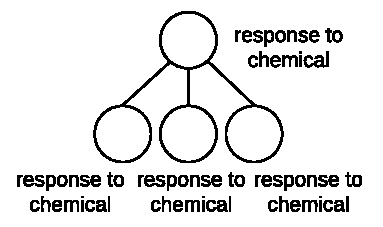
\includegraphics[scale=0.5]{img_ex/proc_1.pdf}
	\caption{Pattern $Q_3$}
		\label{fig:p1}
	\end{subfigure}%
% \captionsetup[subfigure]{labelfont=bf,textfont=normalfont,singlelinecheck=on,justification=raggedright, skip=-5pt}
	\begin{subfigure}[b]{0.30\textwidth}
		% \centering
		\hspace*{10mm}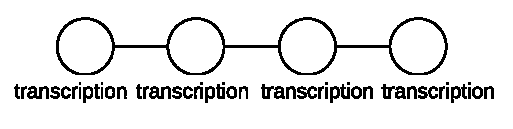
\includegraphics[scale=0.6]{img_ex/proc_2.pdf}
		% \vspace{-4.5mm}
		\caption{Pattern $Q_4$}
		\label{fig:p2}
	\end{subfigure}
	%
	% \begin{subfigure}[b}
	% 	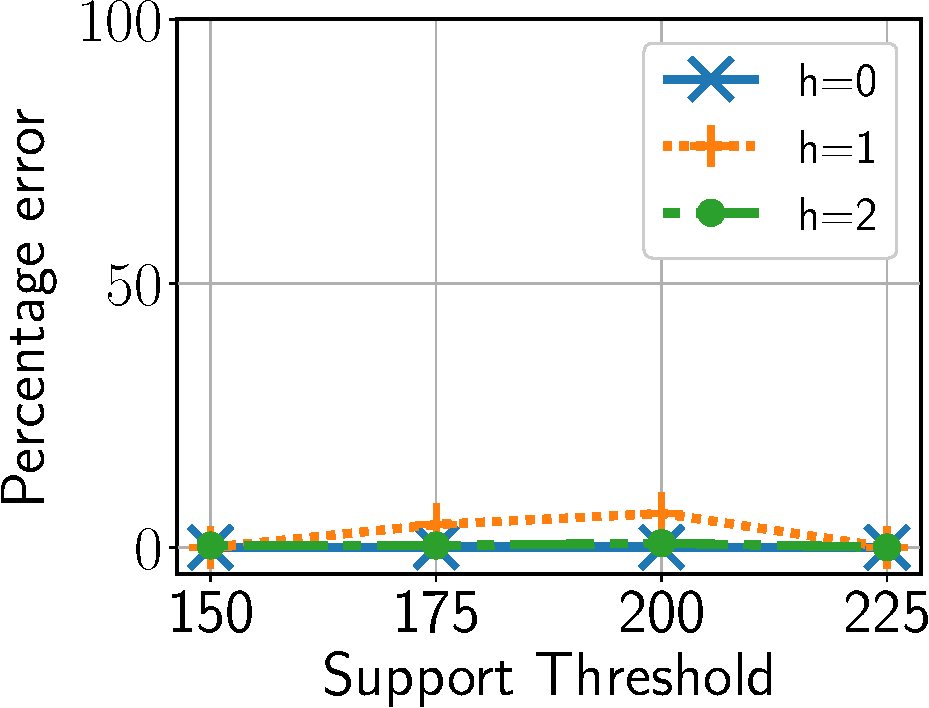
\includegraphics[keepaspectratio,scale=0.24, angle=0]{img2/citeseer/citeseer_spread.pdf}
	% 	\caption{\scriptsize {\sf K}=$20$ in {\em Citeseer}}
	% 	\label{fig:citeseer_error}
	% \end{subfigure}
	\caption{Correlated Subgraph Pairs $(Q_1,Q_2)$ and $(Q_3,Q_4)$}
	\label{fig:yeast}
	% \vspace{-2mm}
\end{figure}

% \spara{$\bullet$ Further Analysis} We provide some further analysis. This part contains the result of the optimization of changing collection tree root in Section \ref{subsubsec:recursive}, and the time cost we spend to avoid the subgraph/supergraph correlations. According to the experimental result, the time we use to prune the not interesting correlations is about 10\% of the total time. Besides, the root changing optimization in Section \ref{subsubsec:recursive} increase the time efficiency by 10\%.


% \begin{figure}[t!]
% \vspace{4mm}
% \centering
% \subfigure[{\scriptsize {\em DBLP} with {\sf Min-sup} = $5000$, $h=2$}] {
% \includegraphics[scale=0.17, angle=270]{addimg/opt_dblp}
% \label{fig:opt1}
% }
% \subfigure[{\scriptsize {\em LastFM} with {\sf Min-sup} = $200$, $h=2$}]  {
% \includegraphics[scale=0.17, angle=270]{addimg/opt_lastfm}
% \label{fig:opt2}
% }
% \vspace{-2mm}
% \caption{\scriptsize Figure for further analysis.}
% \label{fig:opt}
% \vspace{-2mm}
% \end{figure}


% \spara{$\bullet$ Approximation Algorithm Analysis.} We provide the experimental result of our approximation mining algorithm.


% \begin{figure}[t!]
% \vspace{4mm}
% \centering
% \subfigure[{\scriptsize {\em DBLP} with {\sf Min-sup} = $5000$}] {
% \includegraphics[scale=0.17, angle=270]{addimg/a_dblp}
% \label{fig:ap1}
% }
% \subfigure[{\scriptsize {\em LastFM} with {\sf Min-sup} = $200$}]  {
% \includegraphics[scale=0.17, angle=270]{addimg/a_lastfm}
% \label{fig:ap2}
% }
% \vspace{-2mm}
% \caption{\scriptsize Figure for approximation algorithm analysis.}
% \label{fig:ap}
% \vspace{-2mm}
% \end{figure}



% \begin{figure}[t!]
% \vspace{-2mm}
% \centering
% \subfigure[{\scriptsize FSM on {\em Chemical}}] {
% \includegraphics[scale=0.17, angle=270]{img2/fsm_chemical}
% \label{fig:grami1}
% }
% \subfigure[{\scriptsize FSM on {\em Yeast}}]  {
% \includegraphics[scale=0.17, angle=270]{img2/fsm_yeast}
% \label{fig:grami2}
% }
% \subfigure[{\scriptsize FSM on {\em DBLP}}] {
% \includegraphics[scale=0.17, angle=270]{img2/fsm_dblp}
% \label{fig:grami3}
% }
% \subfigure[{\scriptsize FSM on {\em LastFM}}]  {
% \includegraphics[scale=0.17, angle=270]{img2/fsm_lastfm}
% \label{fig:grami4}
% }
% \subfigure[{\scriptsize a subgraph with 8 auto-morphisms}]  {
% \includegraphics[scale=0.3]{img2/grami5}
% \label{fig:grami5}
% }

% \vspace{-2mm}
% \caption{\scriptsize Comparison with {\sf GRAMI}.}
% \label{fig:grami}
% \vspace{-6mm}
% \end{figure}


% \spara{$\bullet$ Comparison with {\sf GRAMI}.} Additionally, we provide the efficiency analysis of the problem, frequent subgraph mining (FSM), of our approach {\sf CSM}, compared with the state-of-art approach of FSM in a single large graph, {\sf GRAMI}\cite{EASK14}. As the state-of-art FSM algorithm in a single large graph, {\sf GRAMI} transforms the subgraph isomorphism to a CSP (constraint satisfaction problem) and makes optimization based on it. Corresponding to our experiment result, in most of the conditions, {\sf GRAMI} has a higher efficiency due to that it does not need to find all the occurrances. However, {\sf GRAMI} could not a good performance dealing with some subgraphs since the most significant optimization, push-down prunning, could hardly contribute in this case (All the positions are valid domains of the subgraph pattern and there are totally $8$ isomorphisms using MNI metric in Figure \ref{fig:grami5}).
